%!TEX root = ../dissertation.tex
\chapter{Experiments}

All of the following experiments were executed on a commodity laptop, a MacBook Air with a 1.4 GHz Intel Core i5 processor and 8GB of RAM.
The lowend nature of our platform illustrates the potential ubiquity of using discrete optimization techniques.
In addition, we hope that this accessibility will allow our model to be used in places without advanced computing resources such as police departments, courts, and hospitals.

We first examine the accuracy of our algorithm on each of our datasets and compare it to other interpretable and non-interpretable methods.
Then, we demonstrate that without our algorithmic and data structure improvements, it would be intractable to solve a real-world problem.
We also show that even with our improvements, this algorithm would not have been able to be run just 25 years ago.
Next, we examine the improvements made to our symmetry-aware map to reduce the memory overhead on our algorithm.
Finally, we describe a parallel implementation and some of the issues that complicate a parallel implementation.

\begin{figure}
\vspace{-2cm}
\begin{center}
\begin{minipage}{\textwidth}
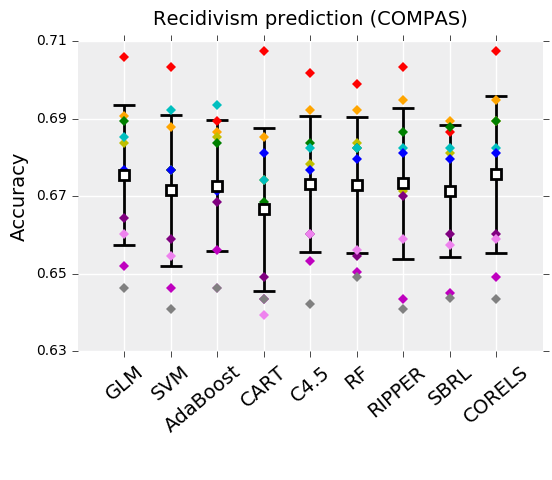
\includegraphics[width=0.8\textwidth]{figs/compas_accuracy.png}
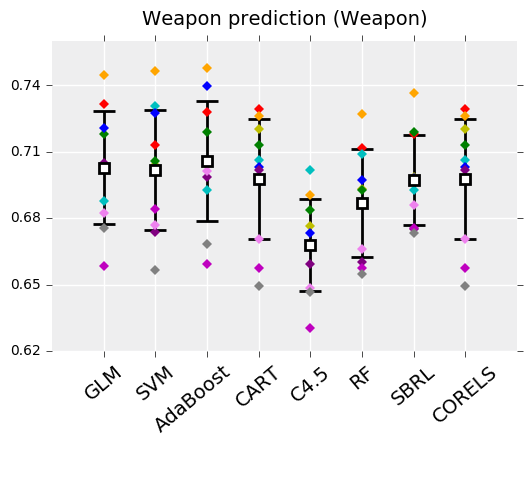
\includegraphics[width=0.8\textwidth]{figs/weapon_accuracy.png}
\vspace{-1cm}
\caption{10-fold cross validation of various machine learning models on the COMPAS and Weapon datasets.
CORELS performs as well as or better than equivalent interpretable and black-box models.
Method type from left to right: Logistic Regression, Support Vector Machine, Boosted Decision Tree, Decision Tree, Decision Tree, Random Forest, (Rule Set), Rule List, Rule List}
\end{minipage}
\end{center}
\label{fig:accuracy}
\end{figure}
%\afterpage{\clearpage}
\section{Accuracy}
We tested CORELS for accuracy on the COMPAS and Weapon datasets.
In addition to CORELS, we tested other interpretable rule based methods such as RIPPER and SBRL, tree methods such as CART, C4.5, and Adaboost, and less interpretable algorithms such as random forests, logistic regression, and SVMs.
Fig \ref{fig:accuracy} shows that CORELS performs just as well as any other predictive method that we tested on the COMPAS and Weapon datasets.
Both of these problems are difficult, so no model is able to capture all of the nuances of human behavior perfectly.
We see that CORELS performs slightly better than other rule based methods such as SBRL and RIPPER \cite{YangRuSe16}, but that these other methods are not far from optimal.
In addition, we see no increase in accuracy granted by using a non-interpretable method instead of an interpretable method such as CORELS.
This provides evidence against the claim that predictive accuracy on these problems will suffer if an interpretable algorithm is used.

\begin{figure}[t!]
%\vspace{-3mm}
\begin{algorithmic}
\normalsize
\State \textbf{Optimal COMPAS rule list}
\State \bif $(age=23\text{--}25) \wedge (priors=2\text{--}3)$ \bthen $yes$
\State \belif $(age=18\text{--}20)$ \bthen $yes$
\State \belif $(sex=male) \wedge (age=21\text{--}22)$ \bthen $yes$
\State \belif $(priors > 3)$ \bthen $yes$
\State \belse $no$\\

\State \textbf{Optimal Weapon rule list}
\State \bif $stop\text{ }reason=suspicious\text{ }object$ \bthen $yes$
\State \belif $location=transit\text{ }authority$ \bthen $yes$
\State \belif $stop\text{ }reason=suspicious\text{ }bulge$ \bthen $yes$
\State \belse $no$
\end{algorithmic}
%\vspace{-3mm}
\caption{Above: The optimal rule list that predicts two-year recidivism for a fold of the COMPAS dataset, found by CORELS.
Below: The optimal rule list that predicts whether or not someone who is stopped by the NYPD has a weapon for one fold of the Stop and Frisk dataset, found by CORELS.}
\label{fig:rule-list-optimal}
\end{figure}

%TODO add sentence about how previous crimes could be racially biased because of criminal justice system
Fig \ref{fig:rule-list-optimal} shows that neither the optimal rule list for COMPAS nor the one for Weapon includes a race related rule.
Both datasets were mined for rules pertaining to race, which means that those rules were not predictive enough to be in the optimal rule list.
This shows that it is possible to get models with state of the art accuracy that do not rely on race to make their predictions.
Thus, the excuse that using a racially biased model is more predictive does not hold true.
These rule lists are short and accurate and therefore would be useful as a racially unbiased heuristic aid for judges and police officers.

\section{Isolated Component Analysis}
We wished to determine how helpful each theoretical bound and data structure optimization was.
We ran a number of experiments where we took out a single component from our system and measured the effects on the runtime and memory usage of our algorithm.
We find that the equivalent points bound is our most important optimization for running in a reasonable amount of time.
Each other optimization and bound plays an important, but not crucial, role in the speed of our algorithm.

In addition, we wanted to find out how much of an overall speed-up CORELS gave compared to a naive implementation.
On the COMPAS dataset, where $n = 155$, naively evaluating all prefixes of up to length 5 would require examining 84,382,025,575 different prefixes.
However, with our solution, we examine only 99,891,878 prefixes in total---a reduction of 845x.
Note that this is a lower bound on the reduction since any brute force solution would have to examine prefixes of longer than length 5 to certify optimality.
It takes us about 2$\mu$s to evaluate a single prefix.
Thus, a naive solution would take 168,764s---about 2 days---while CORELS takes only 2 minutes.
While the naive solution will eventually complete for this dataset, it is clear that brute force wouldn't scale to larger problems.

However, if we look at how processor speeds have changed over the last 25 years, we can see that computers are about 1,000,000 faster now than they were in 1993. \cite{Supercomputer}
Even with our algorithmic and data structural improvements, CORELS would have taken over 120,000,000s in 1993---an unreasonable amount of time.
Our advances are only meaningful because we can run them on a modern system.
When we combine our algorithmic improvements with the increased processor speeds,we see that our algorithm runs almost 1 billion times faster than a naive implementation would have in 1993.
%Nov 2016 125,435.9 TFlops/s
%June 1993 131.0 GFlops/s

\begin{figure}
\begin{center}
\begin{minipage}{\textwidth}
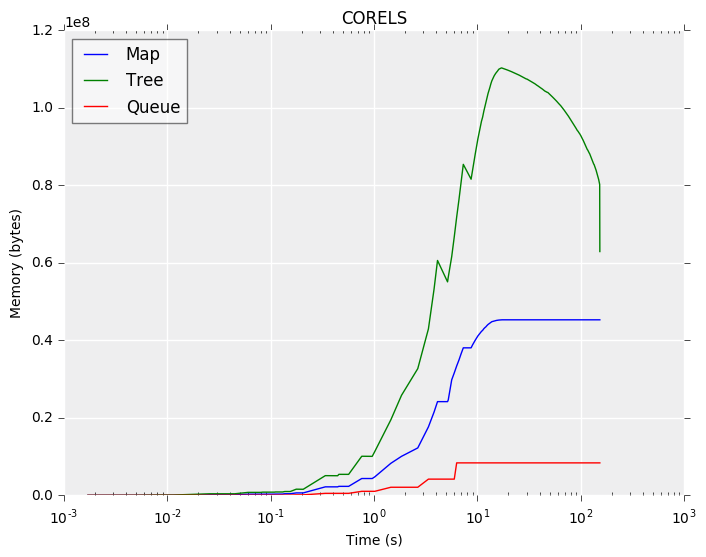
\includegraphics[width=0.9\textwidth]{figs/corels_mem.png}
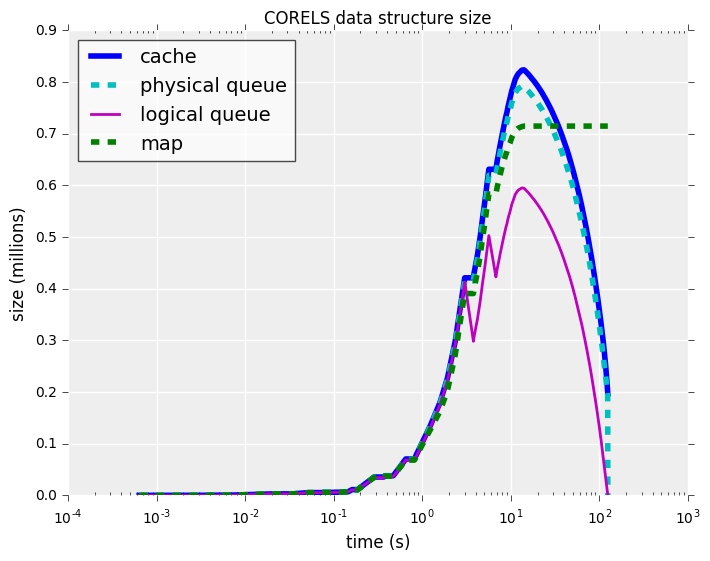
\includegraphics[width=0.9\textwidth]{figs/corels_size.png}
\caption{Memory usage of full CORELS system on the COMPAS dataset. 
Our prefix tree accounts for the bulk of the memory usage.
The size (in number of items) of each of our main data structures.
Corresponds to the amount of memory used.}
\end{minipage}
\end{center}
\label{fig:corels-mem}
\end{figure}

\subsection{Full CORELS system}

Our baseline system with all of our improvements is the CORELS system.
Running the full CORELS system on the Weapon dataset yields the optimal solution and certificate within 142s.
COMPAS is slightly faster, allowing us to discover and certify optimality within 124s.
Fig \ref{fig:corels-mem} shows the growth of our data structures and memory usage throughout the execution of our algorithm.
The maximum memory usage is 170MB, with the majority of that coming from our prefix trie.
With about 1 million items active at the peak, this comes out to about 170 bytes per item.
This includes copies of that item that are kept across the prefix trie, symmetry-aware map, and queue.
For a modern machine, this is not very much memory, demonstrating further that our algorithm can be run without undue memory pressure.

We also run CORELS on the Weapon dataset, which has fewer rules but many more individuals.
This will cause optimizations that limit the depth of our search---the equivalent points bound, the lookahead bound---to be less important than ones that allow us to prune more aggressively---the priority queue and symmetry-aware map.
This section demonstrates that while individual optimizations may play a larger role in certain datasets, the entirety of the system allows for speedy computation and certification of the optimal solution.

\begin{figure}
\begin{center}
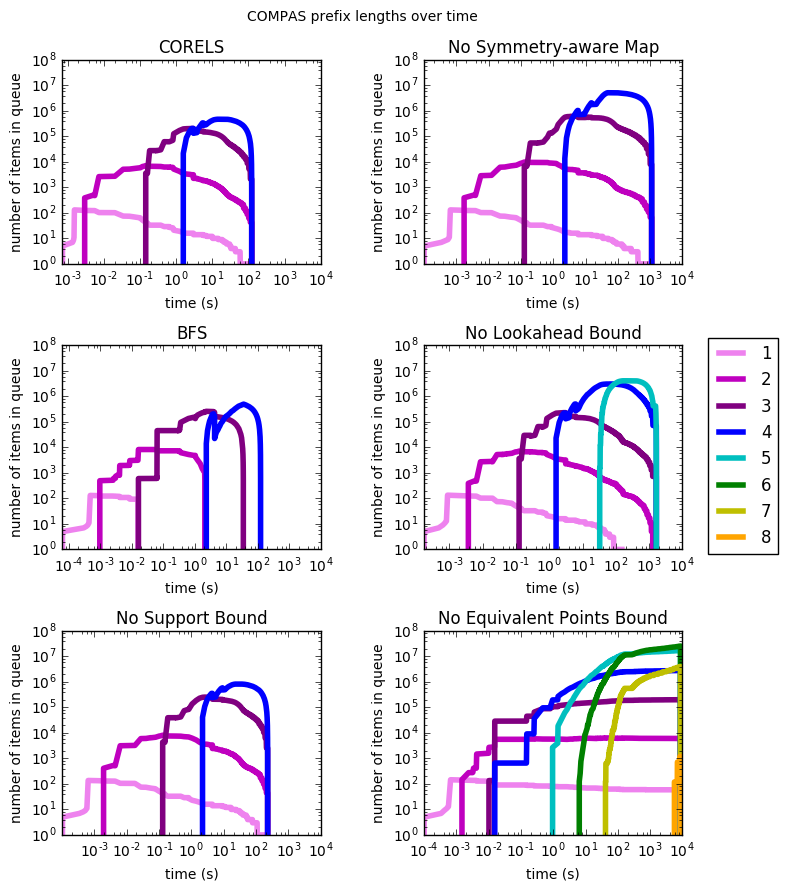
\includegraphics[width=1.1\textwidth]{figs/compas_prefixes.png}
\end{center}
\caption{Tracks the number of prefixes of a given length active in the queue for our system when running on the COMPAS dataset.
Each graph represents an experiment run without one of our bounds or data structures.
This allows us to isolate the critical improvement(s) for a given class of problem.
The equivalent points bound is especially important for datasets with a large number of rules and relatively few data points.
}
\label{fig:compas-prefixes}
\end{figure}

\begin{figure}
\begin{center}
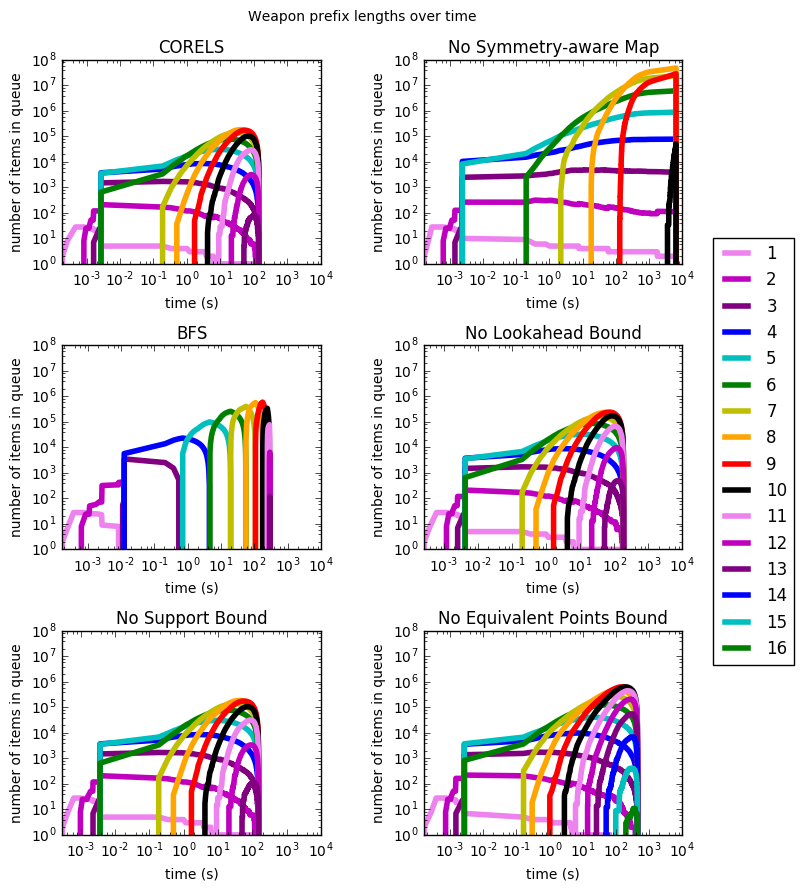
\includegraphics[width=1.1\textwidth]{figs/weapon_prefixes.png}
\end{center}
\caption{Tracks the number of prefixes of a given length active in the queue for our system when running on the Weapon dataset.
Each graph represents an experiment run without one of our bounds or data structures.
This allows us to isolate the critical improvement(s) for a given class of problem.
The symmetry-aware map and permutation bound are especially important for datasets with few rules but a lot of data points.
}
\label{fig:weapon-prefixes}
\end{figure}

\subsection{Priority Queue} \label{exp:priority}

One of our first optimizations was the use of a priority queue to utilize different exploration techniques. 
On the COMPAS dataset, using BFS instead of a priority queue does not seem to harm our performance at all, 
Removing the priority queue from the Weapon dataset, however, and simply using BFS slows down our performance by a factor of 2.
The queue requires very little memory and can give us a significant speed-up on certain types of problems.

\subsection{Support Bounds}

The support bounds are intrinsic to the rules and are the first bounds we check in our execution, because they are the simplest to compute.
Despite this ease of computation, these bounds prevent the pursuit of useless rules.
Without these bounds we complete the certification in 229s (1.8x) for COMPAS and 153s (1.08x) for Weapon.
So, these bounds are not crucial for the completion of our algorithm, but they do provide a nice speed-up.

\begin{table}[t!]
\begin{adjustwidth}{-.4in}{-.4in}
\begin{tabular}{l | c | c | c | c | c | c} 
  Removed component & $t_\text{total}$ (s) & $t_\text{opt}$ (s) & $i_\text{total}$ ($\times 10^6$) & $Q_\text{max}$ ($\times 10^6$) & $K_\text{max}$ & $t/t_\text{CORELS}$ \\
\hline
none (CORELS) & 142 & 0.002 & 1.15 & 0.67 & 13 & 1 \\
priority queue (BFS) & 297 & 0.012 & 2.40 & 0.68 & 13 & 2.09\\
support bounds & 153 & 0.003 & 1.21 & 0.69 & 13 & 1.08 \\
symmetry-aware map & $>$ 6400 & $>$0.002 & $>$114 & $\ge$108 & $\ge$ 10 & $>$45\\
lookahead bound & 186 & 0.004 & 1.56 & 0.9 & 13 & 1.31\\
%equiv. pts. bound & 188.6 (104.6) & 6178 (1840) & 803.8 (0.1) & 790.5 (0.4) & 10-10
equivalent pts bound & 443 & 0.002 & 4.85 & 2.7 & 16 & 3.32
\end{tabular}
\vspace{3mm}
\caption{Per-component performance improvement.
%
The columns report total execution time,
time to optimum, number of queue insertions,
maximum queue size, and maximum evaluated prefix length.
%
The first row shows CORELS; subsequent rows show variants
that each remove a specific implementation optimization or bound.
%
(We are not measuring the cumulative effects of removing a sequence of components.)
%
All rows represent complete executions, except for the symmetry-aware map row,
in which each execution was terminated due to memory constraints
}
\end{adjustwidth}
\label{tab:weapon}
\end{table}

\subsection{Symmetry-aware map}
\label{exp:ablation-pmap}
The symmetry-aware map is a novel way of approaching branch-and-bound, and it plays a large role in our elimination of search space.
Using the symmetry-aware map means that we are able to pursue only one prefix out of all of its permutations.
As our prefixes grow to length 4, for example, that means we can eliminate at least 23 additional prefixes.
For a problem like COMPAS, where we typically examine prefixes up to length 5 (we examine prefixes of length 5 even though Fig \ref{fig:compas-prefixes} only shows prefixes up to length 4 being placed in the queue), this can be a very important bound.
However, we can see the true importance of the symmetry-aware map on the Weapon dataset in Table \ref{tab:weapon} where we are unable to even finish the problem without the symmetry-aware map.
This problem requires us to look at rule lists of length 10 or more, so the permutation bound helps eliminate millions of prefixes.

\begin{comment}
\begin{figure}[t!]
\begin{center}
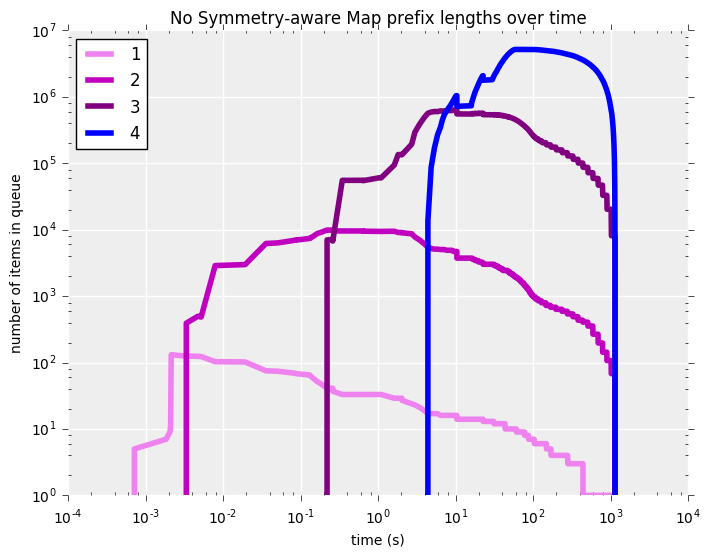
\includegraphics[width=0.9\textwidth]{figs/pmap_prefixes.png}
\end{center}
\caption{Tracks the number of prefixes of a given length active in the queue for CORELS without a symmetry-aware map}
\label{fig:pmap-prefixes}
\end{figure}
\end{comment}

\subsection{Lookahead Bound}
Our lookahead bound is useful for preventing us from examining longer prefixes than we need to.
From running our full CORELS system on COMPAS, we know that our optimal rule list is of length 4.
With our lookahead bound, we never have to place prefixes of length 5 into our queue.
However, removing that bound means that we do place prefixes of length 5 into our queue and therefore have to examine prefixes of length 6.
This drastically slows our computation to 1646s, a 13x slowdown over our full CORELS system.
However, this bound is much less important on the Weapon dataset where we are already examining long rule lists.

\begin{comment}
\begin{figure}[t!]
\begin{center}
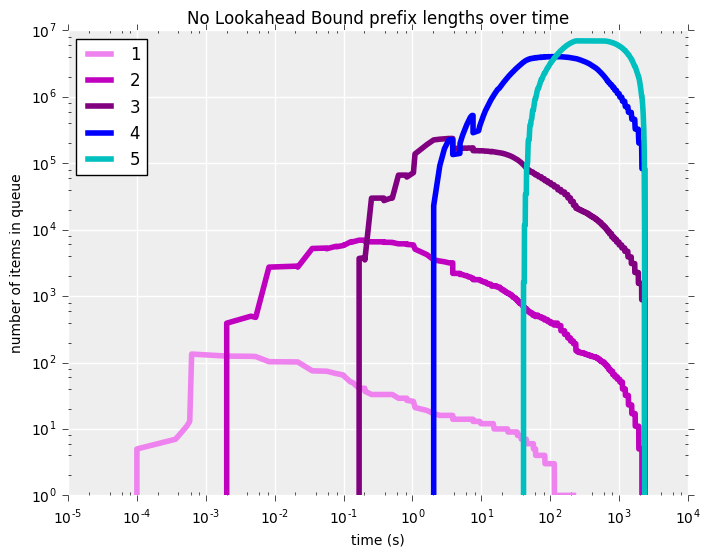
\includegraphics[width=0.9\textwidth]{figs/lookahead_prefixes.png}
\end{center}
\caption{Tracks the number of prefixes of a given length active in the queue without our lookahead bound}
\label{fig:lookahead-prefixes}
\end{figure}
\end{comment}

%\makebox[1.2\textwidth][c]{
\begin{table}[t!]
\begin{adjustwidth}{-.4in}{-.4in}
\begin{tabular}{l | c | c | c | c | c | c} 
  Removed component & $t_\text{total}$ (s) & $t_\text{opt}$ (s) & $i_\text{total}$ ($\times 10^6$) & $Q_\text{max}$ ($\times 10^6$) & $K_\text{max}$ & $t/t_\text{CORELS}$ \\
\hline
none (CORELS) & 124 & 5.6 & 0.84 & 0.59 & 4 & 1.0 \\
priority queue (BFS) & 121 & 4.22 & 0.99 & 0.50 & 4 & 0.98 \\
support bounds & 229 & 9.1 & 1.3 & 0.98 & 4 & 1.8 \\
symmetry-aware map & 1118 & 15 & 6.5 & 5.6 & 4 & 9.0\\
lookahead bound & 1646 & 6.2 & 7.6 & 6.9 & 5 & 13 \\
%equiv. pts. bound & 188.6 (104.6) & 6178 (1840) & 803.8 (0.1) & 790.5 (0.4) & 10-10
equivalent pts bound & $>$8780 & $>$21 & $>$50 & $>$50 & $\ge$8 & $>$ 71
\end{tabular}
\vspace{3mm}
\caption{Per-component performance improvement.
%
The columns report total execution time,
time to optimum, number of queue insertions,
maximum queue size, and maximum evaluated prefix length.
%
The first row shows CORELS; subsequent rows show variants
that each remove a specific implementation optimization or bound.
%
(We are not measuring the cumulative effects of removing a sequence of components.)
%
All rows represent complete executions, except for the final row,
in which each execution was terminated due to memory constraints
}
\end{adjustwidth}
\label{tab:compas}
\end{table}
%}

\subsection{Equivalent points bound}

The equivalent points bound is our optimization that provides the largest benefit when we have a large number of rules.
Since all of our other bounds eliminate prefixes contingent on the lower bound, the equivalent points bound is important because it tightens the lower bound.
Removing this bound typically makes it impractical to complete real world problems.
For COMPAS Table \ref{tab:compas} demonstrates that even after halting execution after multiple hours (8780s), there is still a large portion of the search space to be explored.
This bound plays less of a role for the Weapon dataset, but still remains an important optimization.

\begin{comment}
\begin{figure}[t!]
\begin{center}
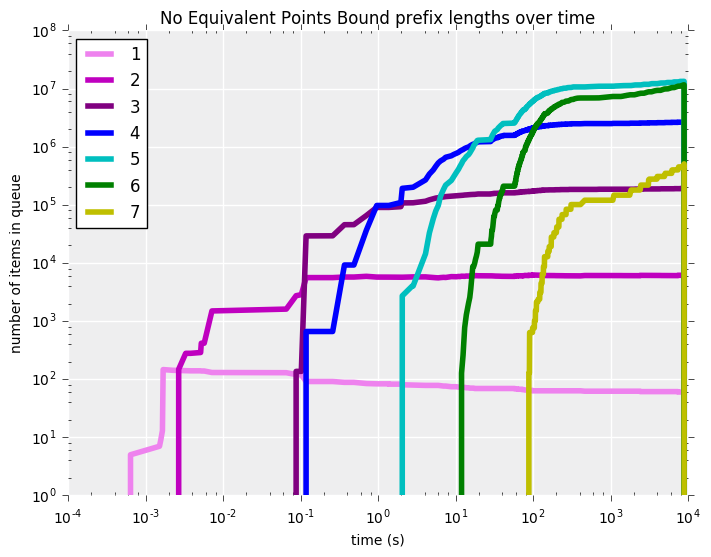
\includegraphics[width=0.9\textwidth]{figs/equivalent_prefixes.png}
\end{center}
\caption{Tracks the number of prefixes of a given length active in the queue without the equivalent points bound}
\label{fig:equivalent-prefixes}
\end{figure}
\end{comment}

\section{Symmetry-aware Map Optimization}
As one of our two main data structures, the memory usage of our symmetry-aware map is something that was very important to us.
In early versions of this algorithm, the symmetry-aware map was the most memory-intensive data structure and we would often run out of memory before certifying the optimal rule list.
Section \ref{exp:ablation-pmap} shows us that running without a symmetry-aware map leads to a much longer runtime, so we needed to find a way to use the symmetry-aware map while reducing memory usage. 
In the course of a normal execution, our permutation map would grow to be hundreds of thousands or millions of entries large.
Thus, carrying a lot of memory overhead with each node led to excess memory usage and ran us out of memory.
This section explores some of the techniques we used to address this memory bloat.

Our first instantiation of the symmetry-aware map was an STL map with keys of type STL sets and values of type a pair of an STL vector and a double.
The first problem is that the STL map is implemented as a red-black tree, meaning every node had the overhead of multiple pointers pointing to its children.
This can be solved using a STL unordered map, which is implemented as a hashtable.
That has some overhead, since it will allocate more buckets than are filled, but it has much less overhead than the two pointers per node of overhead of the STL map.

Our original scheme also used the 8 byte size\_t to represent rule ids.
By assuming that we'll never have more than 65000 rules---which would overtax our algorithm anyways---we were able to use 2 byte unsigned shorts for our rule ids.
This means that our key type, value type, and our node type were able to use only 2 bytes per rule id instead of 8 bytes.
Since our prefixes often get to be length 5 or greater, saving 6 bytes per rule in every representation of the prefix is a large space saving.

\begin{figure}[t!]
\begin{center}
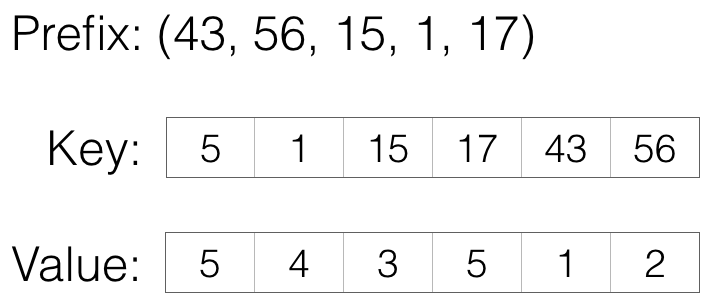
\includegraphics[width=0.9\textwidth]{figs/pmap_types.png}
\end{center}
\caption{An example prefix (43, 56, 15, 1, 17) and the associated representations in the key and the value types.
The key is an array of 6 unsigned shorts where the first entry demarcates the length of the prefix.
Each the rest of the array are the rule ids of the prefix in canonical order.
The value is an array of 6 unsigned chars where the first entry again represents the length of the prefix.
The remaining entries in the array map the rule ids in the canonical order to their actual order in the prefix.
For instance, the first entry in the key is 1 and the first entry in the value is 4, so rule 1 is the 4th rule in the prefix.}
\label{fig:pmap-types}
\end{figure}

After these initial optimizations, we worked on optimizing our key type.
The only criteria for our key type is that two different prefixes that are permutations of each other should map to the same key.
We began by using a STL set as the key because it allowed us to easily determine if two prefixes were permutations of each other by simply inserting into the set.
However, this carries a lot of overhead because a set needs to support insertions, lookups, and deletions in $O(\log n)$ time.
This overhead varies between compilers, but my machine allocated 32 bytes in total for each 2 byte item inserted into the set, plus 24 bytes for the set itself.
For a prefix of length 5, the corresponding key therefore takes up 160 bytes.
Sets support far more operations than we need, though, so we transitioned to a sorted STL vector.
This still allows us to compare prefixes as permutations, and it reduced overhead because a STL vector is essentially just a dynamically resizing array with a little bit of extra bookkeeping information.
This translates to a prefix of length 5 taking up only 40 bytes.
However, STL vectors still support a broader range of operations than we needed because they need to know when to allocate more space.
All we needed was some way to compare the canonical orders and determine if they were the same.
We created a custom key class by allocating a chunk of memory that held the length of the prefix and the sorted order of the ids.
This kept the same idea that the STL vector had in order to compare two prefixes, but it removed the overhead.
In the end, we use only 12 bytes for the key for a prefix of length 5.
An example of the custom key class is shown in Fig \ref{fig:pmap-types}.

We went through a similar process with our values for the symmetry-aware map.
Our only requirement for the values were that they keep track of which prefix was the current best for the given permutation.
We began with a STL vector to keep track of the actual order of the rules in the prefix, but we again wanted to remove the overhead incurred by the fact that STL containers need to support a wider array of operations than we needed.
We reduced our memory usage through a similar technique of what we did with the key type: we moved from a STL vector to a chunk of memory.
However, we realized that we could do even better because we already had the rule ids---all we need in the value was the ordering of those rules.
Since we don't need to represent the rule ids, we can use unsigned chars instead of unsigned shorts to record the actual ordering of the rule ids stored in the key type.
This is shown in Fig \ref{fig:pmap-types}

\begin{table}[t!]
\begin{tabular}{l | c | c | c | c }
Map version & Key version & Value version & Total Memory (MB) & $t_\text{total}$ (s)\\
\hline
Map & Set (size\_t) & STL Vector (size\_t) & 190.7 & 154 \\
Unordered Map & Set (size\_t) & STL Vector (size\_t) & 185.9 & 150 \\
Unordered Map & Set  (unsigned short) & STL Vector (unsigned short) & 148.6 & 148 \\
Unordered Map & STL Vector (unsigned short) & STL Vector (unsigned short) & 68.7 & 147 \\
Unordered Map & Custom Key & Custom Value & 62.9 & 139 \\
\end{tabular}
\vspace{4mm}
\caption{Symmetry aware map improvements when running on the COMPAS dataset.
%
The columns report the type of map,
type of key, type of value,
total memory used by the symmetry-aware map, and time of execution.
%
Each row represents a different version of the symmetry aware map that we tested.
We see that each optimization reduced the total memory consumption while maintaining or slightly reducing the overall runtime.
}
\label{tab:pmap}
\end{table}

In total, Table \ref{tab:pmap} shows us that these improvements give us a 3x memory reduction on this problem.
These reductions take the symmetry-aware map from being the largest data structure to being smaller than the prefix trie.
Reducing the memory footprint of CORELS was helpful for running on COMPAS, but on larger problems this memory improvement is even more pronounced.

In Section \ref{sec:pmap} we described two different key types for the symmetry-aware map, but all of the above optimizations pertained only to the PrefixKey type.
Dealing with the CapturedKey type required a different approach.
We used the bit vector manipulation library from Yang et al. \cite{YangRuSe16} which was built on top of the GMP library.
These bit vectors are of the GMP defined type mpz\_t, which stands for multiple precision integer.
This type allows us represent and perform operations with very large bit vectors in an efficient manner.
Since unordered\_map is implemented as a hash table, it requires a custom hash for non built-in types.
We initially wrote a function to convert between mpz\_t and a $std::vector<bool>$ so that we could use STL's built-in hash function.
This conversion turned out to be very slow, especially when we were running on data sets with many samples.
These mpz\_t types were fairly large, so copying the information from one place to another was inefficient and impractical.
Instead, we adapted the sdbm hash function to our mpz\_t type. \cite{HashFunctions}.
Once we used our own hash function and didn't have to copy between types, CapturedKeys became much faster.
However, as Fig \ref{fig:prefix-captured} showed, they were still less space efficient that PrefixKeys so we did not pursue them further.

%TODO Integrate
\begin{figure}[t!]
	\begin{center}
	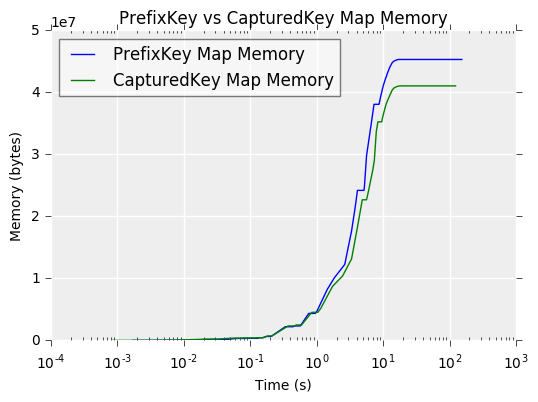
\includegraphics[width=0.8\textwidth]{figs/prefix-captured_pmap_mem.png}
	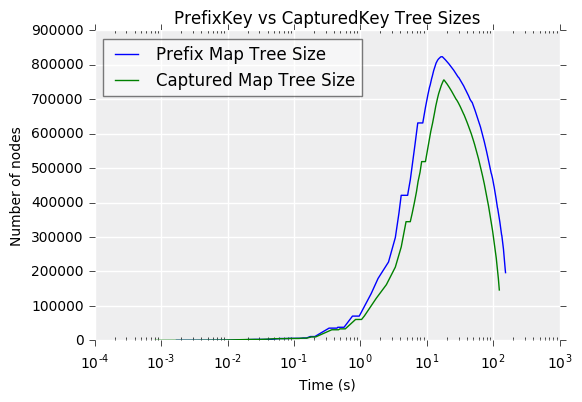
\includegraphics[width=0.8\textwidth]{figs/prefix-captured_tree_size.png}
	\caption{This graph shows the memory usage of the map when using CapturedKeys and PrefixKeys. 
We see that CapturedKeys provide minimal space savings over PrefixKeys due to the slight decrease in nodes inserted into the trie.}
	\end{center}
\label{fig:prefix-captured}
\end{figure}

Indeed, in Fig \ref{fig:prefix-captured}, we find that this occurs in only a few cases, so the size of the map is mostly consistent across different key types.
As can be seen, CapturedKeys are much more memory intensive than PrefixKeys because they're storing all of the data points instead of just a few rules, so we used PrefixKeys for our later analyses.

%TODO add icache statistics and provide #'s for performance deltas
\section{Templates vs Inheritance}
Our system has a lot of different modular parts--various priority metrics, symmetry-aware map types, and different types of information stored in trie nodes.
Since we were using C++, we took advantage of its templating system to achieve this modularity.
We believed that it would be the easiest way to switch out different components of the system, but did not think about the ramifications of this choice.
Due to code duplication, templates can lead to a much larger executable.
Indeed, with a pure templating system, our executable was 253,732 bytes.
Execution time took about 126s on the COMPAS data set.

An alternative way to maintain modularity was to take advantage of C++'s class system and use inheritance and polymorphism.
Instead of having a template argument for each data structure, we can have a base data structure type and then implement each of our extensions as subclasses.
Therefore, we can write all of our functions to take the base class as arguments and then pass in the specialized subclasses based on command line arguments.
This requires the use of virtual functions, which are potentially a bit slower than regular functions, because they require a vtable lookup.
A vtable, or virtual method table, is how C++ deals with the fact that the compiler might not know what class a variable is at compile time, so at runtime the vtable is used to run the appropriate function.
With a pure inheritance framework, our executable was 171,288 bytes.
However, even with the inheritance framework, the runtime of our algorithm was not significantly different from the template runtime.
Thus, since inheritance provided a much cleaner code base to work with, we decided to switch to an inheritance based framework.

\begin{figure}[t!]
	\begin{center}
	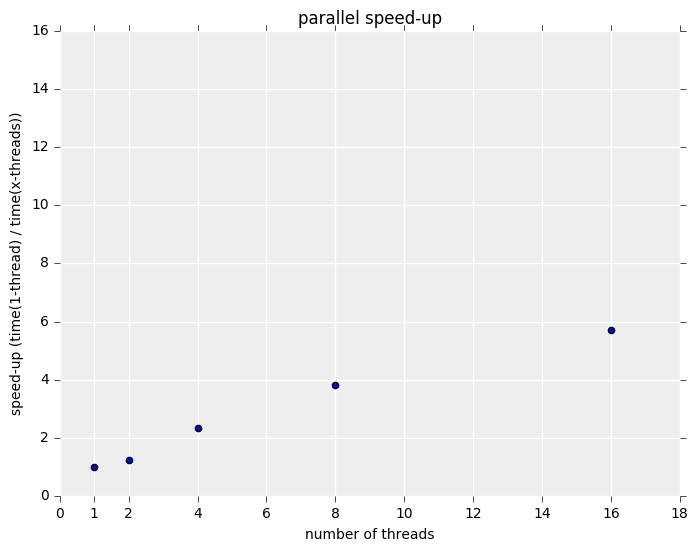
\includegraphics[width=\textwidth]{figs/parallel_speedup.png}
	\caption{This graph shows the speedup of our parallel implementation as we add more threads. 
We see a sub-linear speedup, likely due to cache misses.}
	\end{center}
\label{fig:parallel}
\end{figure}

%TODO Add parallelization graph and finish writing
\section{Parallelization}
Almost every modern machines supports parallelism through the use of multiple cores or simultaneous multi-threading.
This is a crucial fact that modern discrete optimization programs ought to take advantage of.
We show that the structure of this problem nicely supports a parallel implementation of our algorithm.
Furthermore, we show that we get significant, though not linearly-scaling, speed-ups with our parallel implementation.

Analysis of our log files showed that the majority of the time of our program is spent in the incremental section of our execution, shown in Algorithm \ref{alg:incremental}.
So, we began by trying to parallelize this inner loop of our incremental evaluation.
This inner loop involves trying to extend a prefix by calculating the bounds for all possible rules we could add to this prefix.
In order to add these child rules, though, we need to calculate the bounds based on characteristics of the parent prefix.
Without locking the parent, we run into a race condition where one thread is trying to insert a child rule into the parent's representation of the children and another thread is trying to read the parent's representation of the children.
This leads to a segfault in the STL code and could be fixed by locking the appropriate fields in the parent.
%TODO look into this
Locking the parent has too much contention, however, because all of our threads needed to own the parent lock at the same time---essentially rendering the loop sequential.

We realized, however, that the tree structure of our search space, encapsulated in our prefix trie, lends itself nicely to parallelization.
Instead of parallelizing the evaluation of a single prefix, we can parallelize our search over the tree itself.
We do this by creating the tree in the master thread and then spawning worker threads to work in different parts of the tree.
Thus, there is no contention on parents since only one thread can access a node at a time.
The shared state only consists of the minimum objective and the symmetry-aware map, and these are kept in the master thread.
No locking is necessary on the minimum objective because race conditions don't lead to incorrect execution, just to slightly less efficient execution.
For the symmetry-aware map, we lock on insertions and lookups because insertions can trigger a rehash of the underlying hashtable, which is problematic if multiple threads are accessing the map. 
Deletion and garbage collection is handled by the master thread as well.

%TODO find bottleneck and explain
Fig \ref{fig:parallel} shows that parallelizing our implementation did lead to a speed-up, but we see diminishing returns as we increase the number of threads.
One theory we had was that since we had to add locking to the symmetry-aware map, there might be contention that is slowing down the multi-threaded implementation.
However, when we preallocate a large symmetry-aware map and don't lock, we see the same type of slowdown, implying that contention is not the issue.
An alternative explanation is that increasing the number of threads leads to cache thrashing because the appropriate parts of the tree can no longer be kept in memory.